% Source - https://tex.stackexchange.com/a/758849
% Posted by cfr, modified by community. See post 'Timeline' for change history
% Retrieved 2026-02-01, License - CC BY-SA 4.0

\documentclass[tikz,border=5pt]{standalone}
\usetikzlibrary{intersections,spath3}
\begin{document}
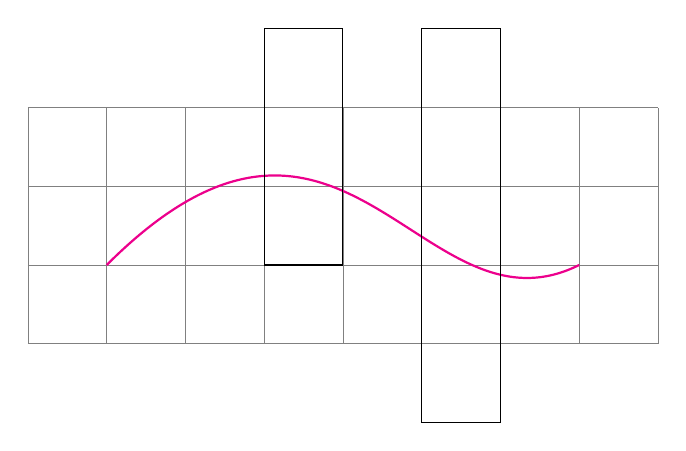
\begin{tikzpicture}
  % based on spath3 manual pp 18-19
  \draw[help lines] (-1,-1) grid (7,2);
  \draw[thick,magenta,spath/save global=Curve] 
  (0,0) .. controls (3,3) and (4,-1) .. (6,0);
  \path [draw,spath/save global=Rectangle] (2,0) rectangle (3,3);
  \path [draw,spath/save global=RectangleB] (4,-2) rectangle (5,3);
  \tikzset{%
    spath/.cd,
    split at intersections={Curve}{Rectangle},
    get components of={Curve}\curveComponents,
  }
%   \draw [line width=3pt,cyan,spath/use=\getComponentOf{\curveComponents}{2}];
  \draw [line width=3pt,violet,spath/use=\getComponentOf{\curveComponentsB}{2}];
\end{tikzpicture}
\end{document}
